%base packages 
\documentclass[11pt]{article}
\usepackage[margin=1in]{geometry}
\usepackage{caption,multirow,etoolbox,color,enumerate,amsmath,dsfont,lscape,tocloft,booktabs,draftwatermark,array,tabularx,graphicx,pdflscape,subcaption}
\usepackage{setspace}
\setlength{\parskip}{0em}
\usepackage[bottom, flushmargin]{footmisc}
\usepackage[T1]{fontenc}
\usepackage[utf8]{inputenc}
\usepackage{lmodern}
\usepackage[english]{babel}
\usepackage[autostyle]{csquotes}
\makeatletter
\makeatother
\usepackage{float}
\SetWatermarkText{}\SetWatermarkLightness{0.85} \SetWatermarkScale{4}
\usepackage{appendix}
\usepackage{authblk}
\usepackage[format=hang,justification=raggedright,singlelinecheck=0,labelsep=period]{caption}
%[format=hang,justification=raggedright,singlelinecheck=0,labelsep=period]
%\usepackage[numbers,sort&compress]{natbib} %Use this set-up for numbered reference lists
\usepackage[authoryear]{natbib} %Use this set-up if you want an un-numbered reference list
%\usepackage{hypernat}

\usepackage[hyperfootnotes=false]{hyperref}
%\usepackage[dvipdfmx,hyperfootnotes=false]{hyperref}
%\usepackage[dvips,hyperfootnotes=false]{hyperref}
\hypersetup{colorlinks=true,linkcolor=blue,anchorcolor=blue,citecolor=blue,filecolor=blue,urlcolor=blue,bookmarksnumbered=true,pdfview=FitB} %
% % %DO NOT PLACE ANY PACKAGES AFTER THE HYPERREF SET UP
\usepackage{titling}

%-----------------------------------------------------------------------%
\begin{document}
\bibliographystyle{mla-good}


\title{Side-Selling and the Returns to Cooperative Participation: The Role of Comparative Advantage in Smallholder Livestock Cooperatives in Nepal}

\author{Scott M. Miller}
\date{}

\sloppy
\maketitle




%------------------------------------------%
\begin{abstract}
Agricultural cooperatives have long been viewed as an important tool for promoting agricultural development and alleviating poverty around the world. Despite this potential, the success of many cooperatives is limited by their inability to successfully coordinate sales and reduce market constraints. This failure is apparent in livestock cooperatives across rural Nepal, where over 80\% of cooperative members engage in side-selling despite the fact that those who sell through the cooperative receive a higher price and sell more goats on average. In order to disentangle this puzzle, I estimate a correlated random coefficient model to analyze the returns to cooperative sales and discuss the importance of comparative advantage in explaining the decision to do so. My results suggest that...
\end{abstract}
%------------------------------------------%

\pagenumbering{gobble}
\clearpage
\renewcommand{\cftsecleader}{\cftdotfill{\cftdotsep}}

\tableofcontents
\clearpage

\doublespacing
\thispagestyle{plain}
\pagenumbering{arabic}
\setcounter{page}{1}

%-----------------------------------------------------------------------%
\section{Introduction} \label{sec:intro}
% Hook
Two-thirds of the world's poorest households live in rural areas and depend on agriculture for their livelihoods \citep{fugile-et.al.19}. Tackling poverty, hunger and malnutrition require drastically increasing the production and commercialization of smallholder agricultural producers \citep{fisher-qaim12,worldbank08}. Although productivity growth in agriculture has the largest impact of any sector on reducing poverty \citep{fugile-et.al.19}, rural markets in developing countries are often rife with constraints that limit the ability of smallholders to sell in formal markets \citep{ashby-et.al.09,kristjanson-et.al.14}. These constraints include poor infrastructure, weak communication channels and long distances between market actors that lead to high transaction costs, weak bargaining power and information asymmetry \citep{aker10,barrett.08,key.et.al.00,staal-et.al.97}. 

In the face of severe market constraints, agricultural cooperatives often arise in an effort to increase bargaining power, decrease transaction costs, and help achieve scale economies in marketing \citep{markelova-et.al.09,rondot-collion01,staal-et.al.97,worldbank03}. By exploiting the potential of collective action, cooperatives provide the opportunity for smallholders to access markets that may otherwise be inaccessible, pool resources to overcome financial constraints, increase communication flows and collectively negotiate with buyers to receive better prices \citep{poole-defrece10}. However, rather than eliminating the source of market constraints, the burdens are shifted to the cooperatives themselves. The effectiveness of cooperatives in raising smallholder market engagement will depend on how well cooperatives manage the challenge of internally coordinating sales among a large group of individual market actors. Evidence suggests that some farmer organizations are able to successfully overcome this challenge, generating large and inclusive benefits for their members \citep{narrod-et.al.09,tadesse-bahiigwa15,wollni-zeller07}. Others largely fail in this effort, resulting in a high presence of side-selling, heterogeneous benefits, or dissolving participation among their members \citep{aflagah-et.al.19,bernard-spielman09, casaburi-macchiavello15}. 

% question
Perhaps the most apparent example of the shortcomings of agricultural marketing cooperatives takes the form of a high presence of side-selling. This phenomena is widespread in livestock cooperatives across rural Nepal, where over 80\% of goat-selling households choose to sell their goats to a local trader instead of through the cooperative of which they are a member. What makes this problem more interesting is that the 20\% of households who sell their goats through the cooperative receive a higher price and sell more goats on average than do the side-selling households.

In order to disentangle this puzzle, I estimate a correlated random coefficient model, following \citet{suri11}, where the adoption choice is to sell through the cooperative rather than to a local trader. By estimating the distribution of net returns to selling through the cooperative, I analyze the role that comparative advantage plays in cooperative participation. My results show that there are [not] significant net returns to cooperative sales, that these returns are [not] heterogeneous and that this heterogeneity [does not] explains the side-selling decision. [Discussion of the role of comparative advantage in cooperative participation decisions.]

% Antecedents
In her seminal paper, \citet{suri11} uses a correlated random coefficient model to explain why, despite high average returns to hybrid maize seed in Kenya, adoption of this technology was persistently low. By accounting for the unobserved heterogeneity of returns to adoption, \citet{suri11} demonstrates that farmers who experience positive benefits adopt the technology, while those who experience low returns choose not to adopt, or disadopt, the technology. Following this methodology, \citet{michler-et.al.18} conduct an extension test of \citet{suri11} in the case of improved chickpea varieties in Ethiopia, and find that there is little heterogeneity in the returns to adoption, and that all groups stand to reduce costs and increase profits from adopting this technology. 

% Value Added
This paper builds on the existing literature in agricultural technology adoption, contract farming and cooperatives in developing countries by estimating a correlated random coefficient model where selling through a local institution (producer cooperatives) is the adoption decision. This approach allows me to analyze the role of comparative advantage at both the farmer and institution levels. This analysis is unique in that it provides an understanding of the characteristics that make farmers and producer cooperatives successful in a development context. 
 

%-----------------------------------------------------------------------%
\section{Background \& Data} \label{sec:background}

In Nepal, where 68 percent of the population depends on agriculture for their livelihood \citep{ILO16}, goats are a common source of income and nutrition. This is particularly true in rural areas, where nearly every household owns a least a few goats for production and/or consumption \citep{upreti09}. In recent years, urbanization and rising incomes have lead to a higher demand for goat meat, but a poorly functioning value chain has left smallholder producers, most of whom are women, unable to benefit \citep{ashby-et.al.09,choudhary-et.al.11,gurung-et.al.15}. Smallholders face high transaction costs, weak bargaining power and a lack of communication infrastructure that limit their ability to access and gain from formal output markets \citep{ashby-et.al.09,kristjanson-et.al.14}. As a result, domestic production has been unable to keep up with rising demand, leading to higher imports from India and Tibet \citep{HI-N12}.

Many agricultural policy and rural development plans in Nepal have promoted agricultural cooperatives as a means of supporting smallholder producers \citep{ADS15}. Non-governmental organizations, including Heifer Project International in Nepal (HPIN), have made recent efforts to strengthen the goat value chain by organizing producer cooperatives. HPIN’s programs give women livestock and extensive training. Beneficiaries are then organized into self-help groups (SHGs) of around 20-30 female members. Once SHGs in a given area are sufficiently organized, they are combined into larger producer cooperatives \citep{janzen-et.al.18}.

% This follows closely from the VCC Pre-Analysis Plan. In the full dissertation, I will cite this accordingly if that paper moves forward
The majority of goats in Nepal are consumed after sale to a local collector who pools animals from smallholder producers \citep{HI-N12}. For goats that are marketed outside of their original communities, the commercial value chain links producers, local collectors and regional traders to consumers who are primarily located in urban markets \citep{HI-N12}. A collector looking to buy goats from smallholder producers who are not affiliated with a cooperative would likely have to conduct individual negotiations, sometimes making multiple visits per home \citep{HI-N12, staal-et.al.97}. After agreeing to terms with producers, the collector would still have to coordinate transportation. If the collector does not want to transport goats from each individual home, then he or she would have to arrange for producers to bring their animals to a collection point at a specific date and time. Bargaining with many small producers and managing logistics may inflate transaction costs and dissuade collectors from dealing with smallholders. In contrast, a collector purchasing through a cooperative need only negotiate with a single entity and can leave sales coordination to cooperative managers.

%-----------------------------------------------------------------------%
\subsection{Data} \label{sec:data}
The data used in this paper were originally collected as baseline and endline data for a randomized control trial. The sample frame of this dataset is a list of 109 cooperatives spread across four of five development regions in Nepal, specifically the East, Central, West and Mid-Western Development regions. All cooperatives operate in either the low-land Terai or mid-Hills. Figure \ref{map} shows the study area covered in the sample, which includes cooperatives from 24 districts across Nepal. The cooperatives included in the study were selected by HPIN and include all existing livestock marketing cooperatives the organization helped form prior to 2017.

\begin{figure}[!h]
    \caption{Study Area}
    \label{map}
    \noindent \centering 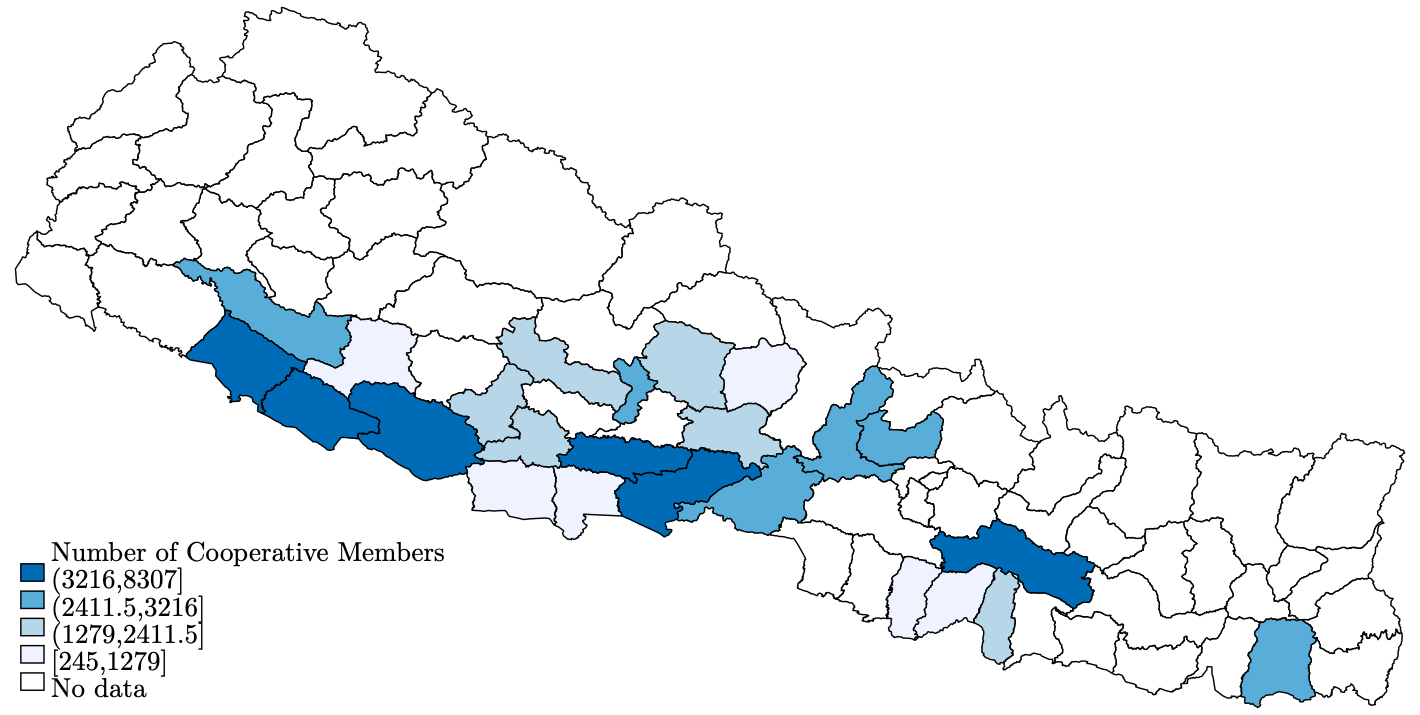
\includegraphics[width=.9\textwidth,trim=4 4 4 4,clip]{StudyMap.png}
\end{figure}

This dataset consists of two separate surveys - one with cooperative leaders and another with general members.  I refer to these surveys as the cooperative leader and household survey, respectively. The cooperative leader survey is comprised of interviews from three officers in each cooperative. To obtain a representative sample for the household survey, HPIN and cooperative leaders generated complete cooperative rosters. From these comprehensive lists, a random sample of 2,856 households across 108 cooperatives was drawn to participate in the household survey. The first round of data were collected from the sample in January 2018 using Android tablets and Open Data Kit. The second round of data was collected in April 2020.

%\newpage
\singlespacing
% Summary Stats Table
\newcolumntype{Y}{>{\centering\arraybackslash}X}
\begin{table}[!h]
  \centering
  \caption{Summary Statistics (2018 Sample)}
  \label{table:summary}
  \scalebox{.8}{
  \begin{tabularx}{1.2\linewidth}{l*{7}{Y}}
\hline Cooperative-Level Variables & N & Mean & sd & Min & Max\\
\noalign{\smallskip}\hline \noalign{\smallskip}
Number of Members (count) & 107.00 & 568.64 & 375.77 & 11.00 & 2,600.00\\
Annual Revenue (USD) & 108.00 & 3,862.05 & 7,503.18 & 0.00 & 65,709.51\\
Annual Costs (USD) & 108.00 & 624.62 & 2,619.28 & 0.00 & 21,383.74\\
Annual Net revenue (USD) & 106.00 & 3,298.52 & 7,929.31 & -16,676.6 & 65,554.2\\
Annual Revenue per member (USD) & 108.00 & 7.26 & 10.34 & 0.00 & 63.53\\
Annual Net revenue per member (USD) & 105.00 & 6.44 & 10.94 & -29.78 & 63.53\\
Annual Goat revenue (USD) & 106.00 & 173.05 & 542.82 & 0.00 & 5,262.24\\
Planning time horizon (years) & 108.00 & 1.33 & 1.07 & 0.00 & 5.00\\
ICT assets (count) & 108.00 & 0.62 & 0.71 & 0.00 & 3.00\\
Non-ICT assets (count) \hspace{2.15in} & 108.00 & 2.85 & 2.36 & 0.00 & 15.00\\


  \end{tabularx}}
  \scalebox{.8}{
  \begin{tabularx}{1.2\linewidth}{l*{7}{Y}}
\hline Household-Level Variables & N & Mean & sd & Min & Max\\
\noalign{\smallskip}\hline \noalign{\smallskip}
Age of female cooperative member (years) & 2,856.00 & 42.35 & 11.58 & 20.00 & 83.00\\
Literacy of female cooperative member (0/1) & 2,856.00 & 0.79 & 0.36 & 0.00 & 1.00\\
Contacted about cooperative sales in last 6-months (0/1) & 2,856.00 & 0.35 & 0.48 & 0.00 & 1.00\\
Total number of goats owned (count) & 2,856.00 & 5.76 & 4.95 & 0.00 & 69.00\\
Household sold goats in the last 12-months (0/1) & 2,856.00 & 0.48 & 0.50 & 0.00 & 1.00\\
Household side-sold goats in the last 12-months (0/1) & 1,384.00 & 0.77 & 0.42 & 0.00 & 1.00\\
Annual number of goats sold (count) & 1,384.00 & 2.31 & 1.85 & 1.00 & 10.00\\
Annual number of cooperative goats sold (count) & 1,384.00 & 0.53 & 1.05 & 0.00 & 4.00\\
Annual revenue per goat (USD) & 1,384.00 & 85.07 & 37.15 & 0.00 & 178.20\\
Annual revenue per cooperative goat (USD) & 353.00 & 91.44 & 30.08 & 0.00 & 135.13\\
Annual net goat income (USD) & 1,384.00 & 148.41 & 159.81 & -284.13 & 725.67\\
\hline
\multicolumn{6}{@{}p{1.2\textwidth}}
{\textit{Notes}: At the household-level, several variables include missing values and are conditional the household selling goats. These variables include: household side-sells goats, total goats sold, cooperative goats sold, revenue per goat and net goat income. Revenue per cooperative goat sold is conditional on the household selling goats through the cooperative.}
  \end{tabularx}}
\end{table}
\doublespacing

Table (\ref{table:summary}) displays summary statistics from the 2018 sample of my data. The average cooperative in my sample has 569 members, and a revenue of over \$3,800 USD. On average, cooperatives operate with a net revenue of roughly \$3,300 USD. However, there is significant heterogeneity in this measure, as average net revenue ranges from below -\$16,600 to more than \$65,500 USD. The average cooperative owns fewer than one information and communication technology (ICT) asset, but owns nearly 3 non-ICT assets. The average cooperative member in my sample is 42 years old, roughly 80\% of whom are literate. While the average household owns more than 5 goats, only 48\% sold a goat in the year prior to data collection and only 35\% received sale information from their cooperative in the 6-months prior to data collection. This may in part explain the disparity between goat sales through and outside of the cooperative. On average, goat-selling households sold more than two goats and received a revenue of \$85.07 USD per goat. Meanwhile, among goat-selling households the average number of cooperative goats sold is 0.53 and the average revenue per cooperative goat sold is \$91.44.

\section{Side-Selling}

Figure (\ref{figure:E2_month}) displays the total number of goats sold through and outside of the cooperative by month in the year prior to round one data collection.\footnote{The calendar year in Nepal begins in mid-April.} This figure shows the extensive presence of side-selling throughout the year, with the number of goats sold outside of the cooperative often more than double the number sold through the cooperative. The highest presence of side-selling occurs during the Nepali festival season (August-December), where there is a spike in the demand for goat meat surrounding holiday celebrations.\footnote{Goat meat is significantly more expensive than many alternatives and is considered a luxury product in Nepal.} This figure indicates that cooperatives are failing to capture the majority of goat sales happening among their membership. 

\vspace{.5cm}
\begin{figure}[H]
    \caption{Total Number of Goats Sold by Sale Channel and Month (2018 Sample)}
    \label{figure:E2_month}
    \noindent \centering 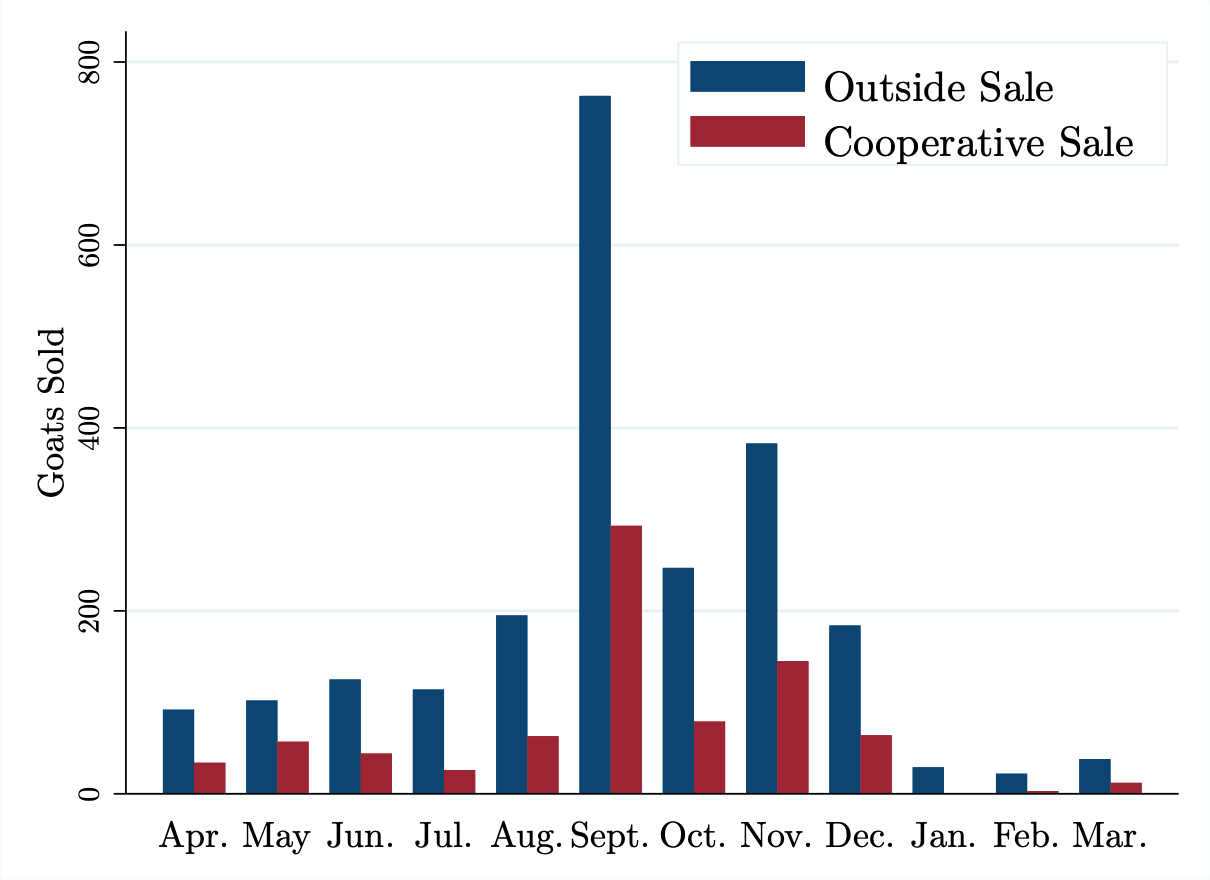
\includegraphics[width=.55\textwidth,trim=4 4 4 4,clip]{E2_SaleMonth.png}
\end{figure}

Figures (\ref{figure:E2_PD_Annual}-\ref{figure:E2_PD_NonFest}) display the distribution of goat prices received through each sale channel for the full calendar year, during festival season and outside of festival season. These figures suggests that selling goats through the cooperative may be more lucrative than side-selling, regardless of the timing of the sale. This further motivates the empirical puzzle that I will investigate in this paper. 

\begin{figure}[H]
\caption{Distribution of Goat Prices by Sale Channel (2018 Sample)}
    \centering
    \begin{subfigure}[t]{.49\textwidth}
    \centering
        \caption{Annual} \label{figure:E2_PD_Annual}
        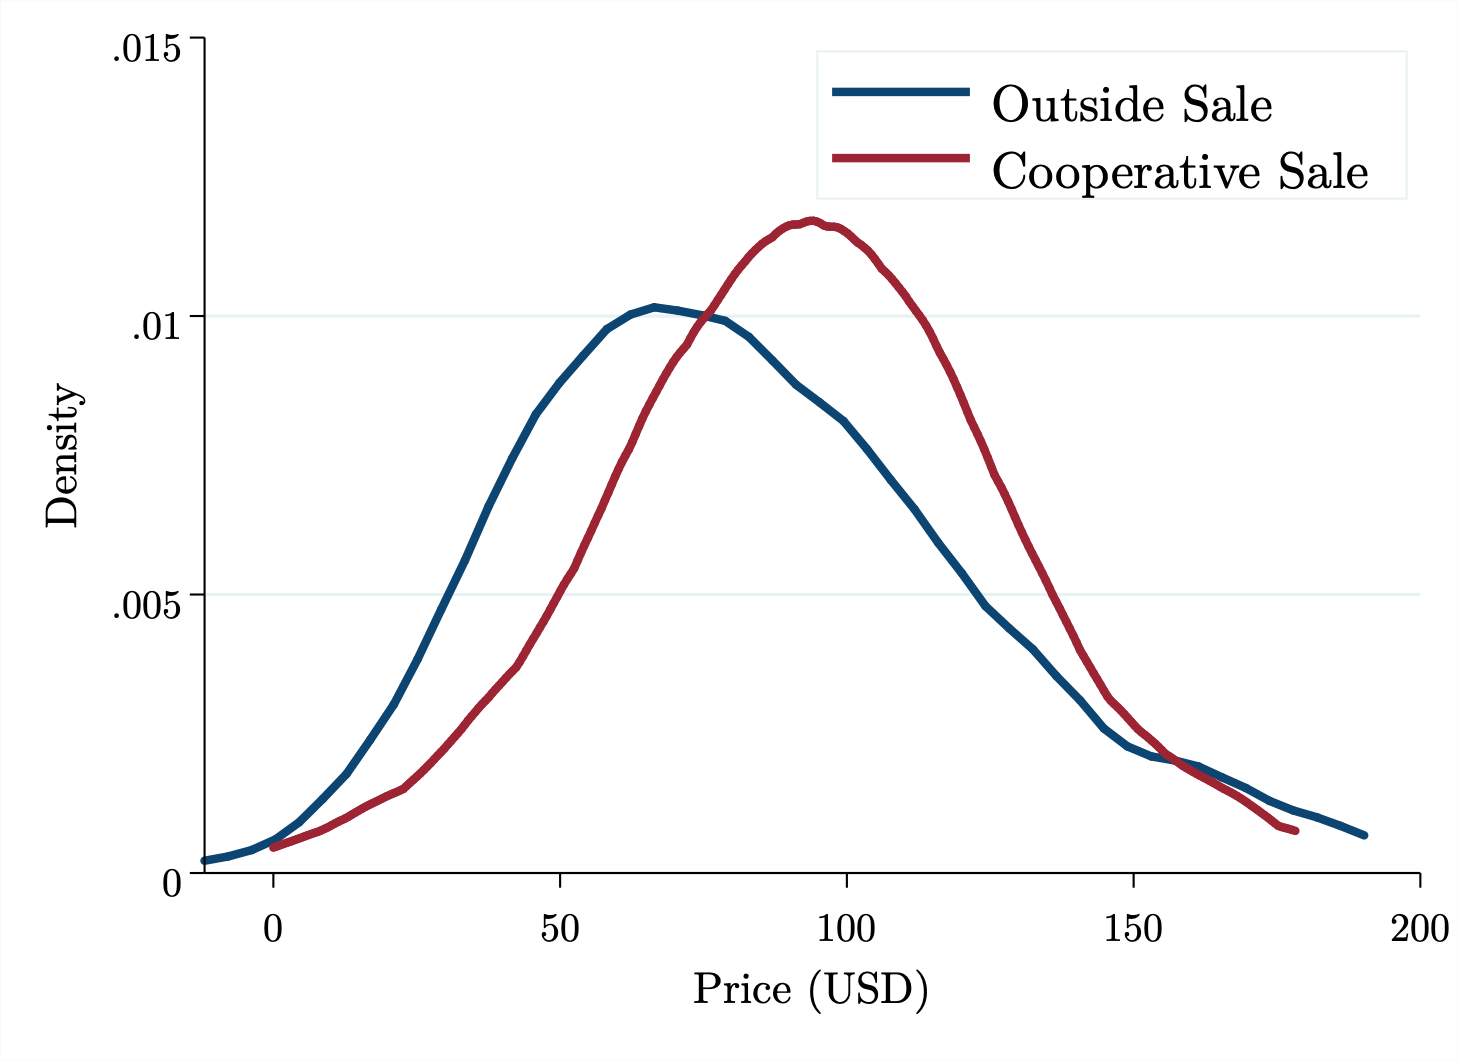
\includegraphics[width=\linewidth,trim=4 4 4 4,clip]{E2_PriceDensity_Annual.png} 
    \end{subfigure}
    \vspace{.5cm}
    \begin{subfigure}[t]{0.49\textwidth}
        \centering
        \caption{Festival Season} \label{figure:E2_PD_Festival}
        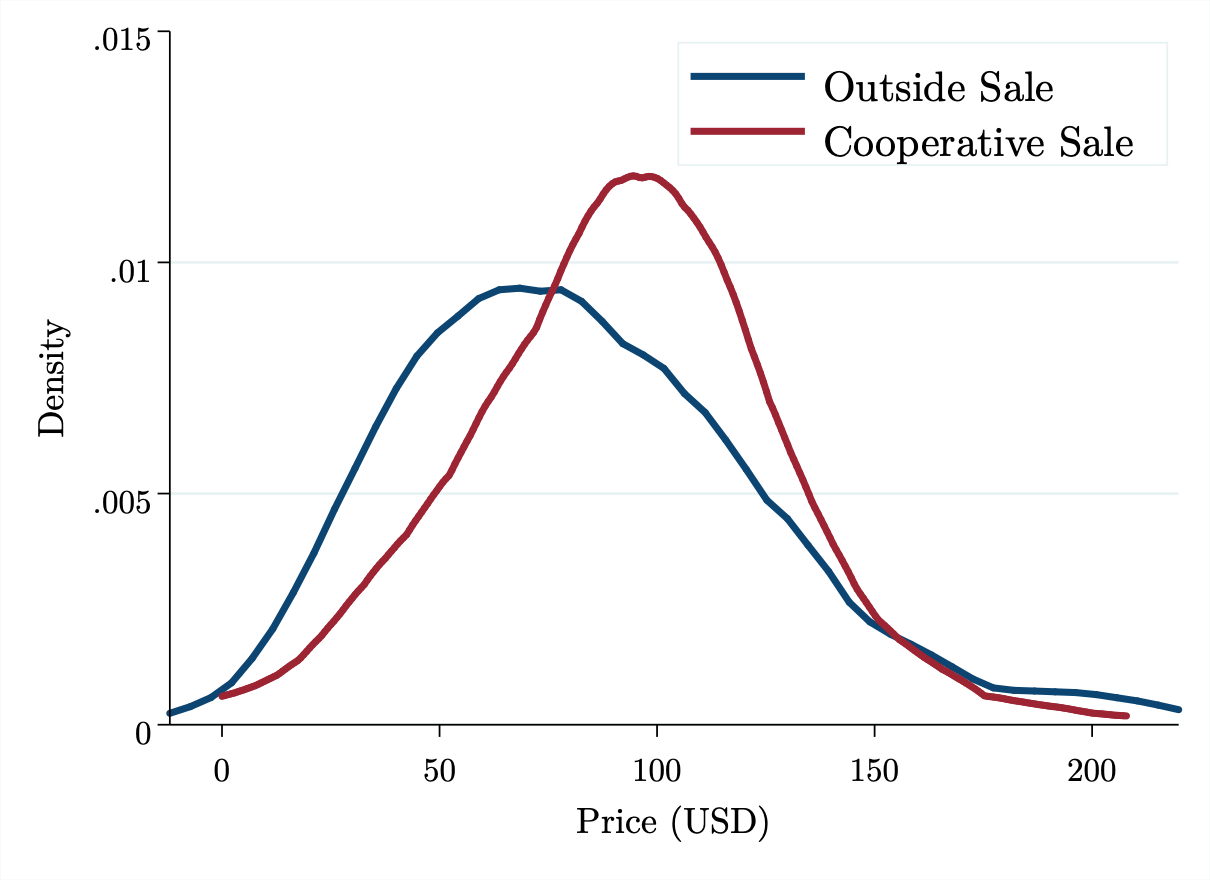
\includegraphics[width=\linewidth,trim=4 4 4 4,clip]{E2_PriceDensity_Festival.png} 
    \end{subfigure}
    \hfill
    \begin{subfigure}[t]{0.49\textwidth}
        \centering
        \caption{Non-Festival Season} \label{figure:E2_PD_NonFest}
        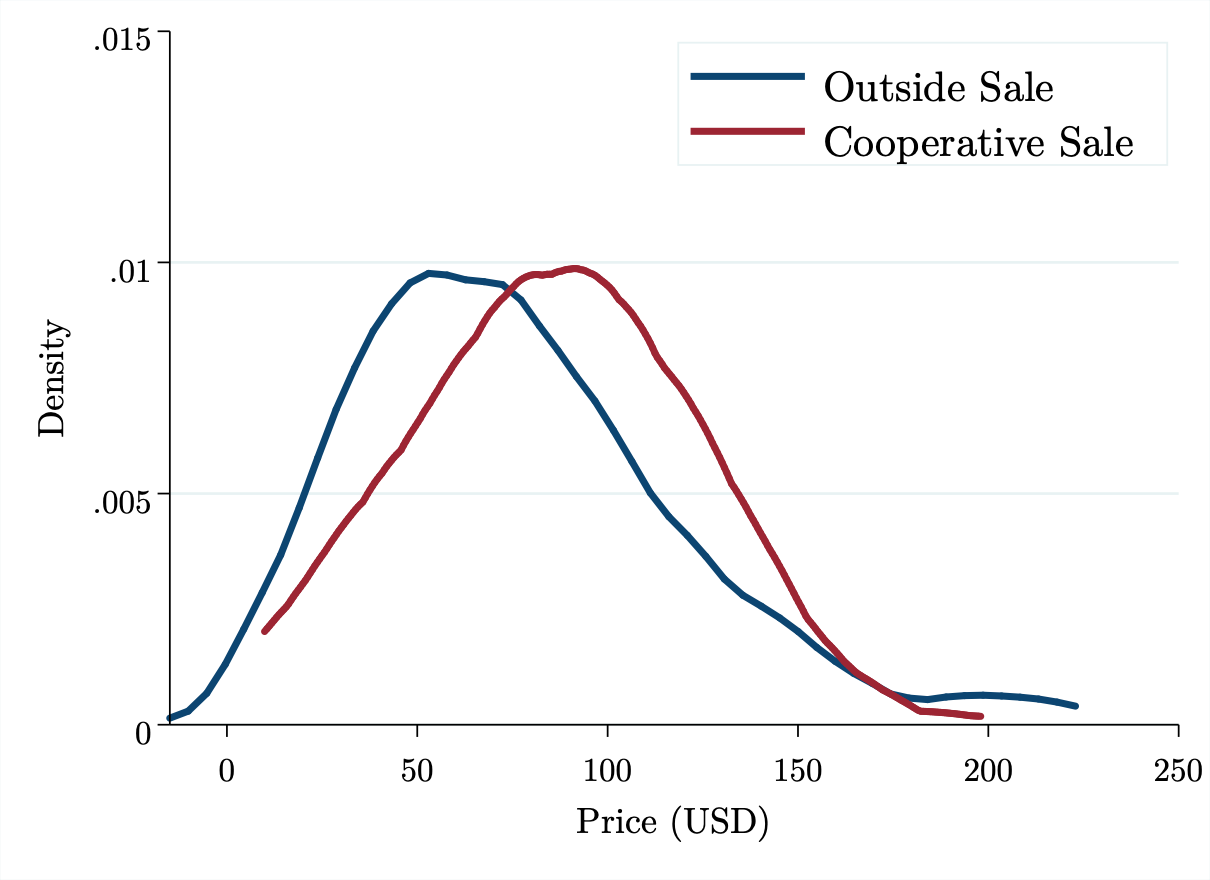
\includegraphics[width=\linewidth,trim=4 4 4 4,clip]{E2_PriceDensity_NonFest.png} 
    \end{subfigure}
\end{figure}


\subsection{Adoption Decisions}

\singlespacing
\begin{center}
\begin{table}[H]
\caption{Transition of Adoption Decisions for the Sample Period} 
\centering
%\vspace{.5cm}
\begin{tabular}{lcccc}
\noalign{\smallskip} \hline \noalign{\smallskip}
 & Adoption & \hspace{-.35cm} Decision & Percent of Sample \\
\noalign{\smallskip} \cline{2-3} \noalign{\smallskip} Group & 2018 & 2020 & (N= ) \\
\noalign{\smallskip} \hline \noalign{\smallskip}
Always adopter & Y & Y & \%  \\ 
Adopter & N & Y & \%  \\
Disadopter & Y & N & \%  \\
Never Adopter & N & N & \%  \\
\hline
\end{tabular}\\
\end{table}
\end{center}
\doublespacing


\begin{table}[!h]
  \centering
  \caption{Reasons for Side-Selling (2018 Sample)}
  \label{table:E2_ss_reason}
  \scalebox{.85}{
  \begin{tabularx}{.9\linewidth}{lcc}
\hline \noalign{\smallskip} & N & \% of households\\
\noalign{\smallskip}\hline \noalign{\smallskip}Delayed payment with cooperative & 1,070.00 & 8.13\\
Cooperative sale point is too far away & 1,070.00 & 18.41\\
Trader offered a higher price & 1,070.00 & 49.72\\
Cooperative did not arrange a sale at this time & 1,070.00 & 29.53\\
\hline
\multicolumn{3}{@{}p{.9\textwidth}}
{\footnotesize{\textit{Notes}: For each sale that was made outside of the cooperative in the year prior to data collection, households were asked to select the option(s) that best represented their decision to side-sell. The percentage of households column reports the percentage of households that selected each option at least once.}}
  \end{tabularx}}
\end{table}
\doublespacing

Table (\ref{table:E2_ss_reason}) reports the reasons that households gave for side-selling in the year prior to round one data collection. For each sale that was made outside of the cooperative in this time-period, households were asked to select the reason(s) that best explain their decision to side-sell. Fewer than ten percent report side-selling due to receiving delayed payments from the cooperative, less than 20\% report doing so because the cooperative's sale point was too far away and nearly 30\% stated that they side-sold because the cooperative did not arrange a sale at the time that they sold goats. Perhaps most important is that nearly half of side-selling households indicate that they sold outside of the cooperative because a local trader offered them a higher price. 

% --------------------------------------
\section{Theoretical Framework} \label{sec:E2_theory}
% rewrite text
Following \citet{michler-et.al.18} and \citet{suri11}, my goal is to estimate the distribution of returns to cooperative goat sales in order to understand if producers are self-sorting into cooperative and outside sales based on whether or not `adopting' is beneficial for them. In order to do this, I estimate the production function that underlies the decision to sell through or outside of the cooperative. I begin by treating the decision to sell through the cooperative as a technology that farmers are able to adopt. While this decision differs from typical agricultural technology adoption decisions, this methodology is useful for understanding the decision-making process around the source of goat sales in this context. Under this framework, producers are faced with the decision to `adopt' (sell through the cooperative), which provides the potential for a higher price and/or a larger number of goats sold, or `not adopt' (sell directly to a local trader), which can be viewed as the standard selling mechanism. The remainder of this subsection closely follows \citet{michler-et.al.18}, and the estimation will be conducted using the Stata package developed by \citet{cabanillas-et.al.18}.

I begin by using a Roy model which assumes that the adoption choice is part of a profit maximization decision, where returns are a function of input costs, output quality and prices. I assume the underlying production function to be Cobb-Douglas and written as
%CM: Consider writing it in log form right away

\begin{equation} \label{eq:E2_yield.C}
    Y^{C}_{it} = e^{\beta^{C}_{t}}\big{(}\prod_{j=1}^{k}X^{\gamma^{C}_{i}}_{ijt}\big{)}e^{u^{C}_{it}}
\end{equation}   
\begin{equation} \label{eq:E2_yield.O}    
    Y^{O}_{it} = e^{\beta^{O}_{t}}\big{(}\prod_{j=1}^{k}X^{\gamma^{O}_{i}}_{ijt}\big{)}e^{u^{O}_{it}}
\end{equation}

%CM: define your subscripts
where $Y^{C}_{it}$ and $Y^{O}_{it}$ are the quantity of goats sold through the cooperative (C) and outside of the cooperative (O), respectively. Yields are a function of inputs ($X^{\gamma^{O}_{i}}_{ijt}$), which can have differential effects on output depending on the adoption decision ($\gamma^{C}_{i}$ and $\gamma^{O}_{i}$). The $\beta$’s are adoption-specific aggregate returns to production, and the $u^{C}_{it}$ and $u^{O}_{it}$ terms are adoption-specific compound error terms, such that

\begin{equation} \label{eq:E2_u.C}
    u^{C}_{it} = \theta^{C}_{i} + \varepsilon^{C}_{it}
\end{equation}
\begin{equation} \label{eq:E2_u.O}
    u^{O}_{it} = \theta^{O}_{i} + \varepsilon^{O}_{it}
\end{equation}

Following \citet{carniero-et.al.15}, \citet{michler-et.al.18} and \citet{suri11}, I assume that households know their own farmer-specific productivity effects, $\theta^{C}_{i}$ and $\theta^{O}_{i}$, but do not know $\varepsilon^{C}_{it}$ and $\varepsilon^{O}_{it}$ prior to the sale. I also assume $\varepsilon^{C}_{it}$ and $\varepsilon^{O}_{it}$ to be uncorrelated with each other as well as with the $X$’s.
As in \citet{lemueux.98}, since $\theta^{C}_{i}$ and $\theta^{O}_{i}$ are unobserved, they can be decomposed into the following productivity effects %CM: The decomposition in 14 and 15 just redefines the variables as a regression. You can write anything as a regression on anything with a zero mean error. Also the thetas have to be mean zero, right? Otherwise you'd have an intercept.

\begin{equation} \label{eq:E2_theta.C}
    \theta^{C}_{i} = b_{C}(\theta^{C}_{i} - \theta^{O}_{i}) + \zeta_{i}
\end{equation}
\begin{equation} \label{eq:E2_theta.O}
    \theta^{O}_{i} = b_{O}(\theta^{C}_{i} - \theta^{O}_{i}) + \zeta_{i}
\end{equation}

where the projection coefficients $b_{C}$ and $b_{O}$ are defined as \singlespacing
$$b_{C} = (\sigma^{2}_{C} - \sigma_{CO}) / (\sigma^{2}_{C} + \sigma^{2}_{O} - \sigma_{CO})$$ 
$$b_{O} = (\sigma^{2}_{O} - \sigma_{CO}) / (\sigma^{2}_{C} + \sigma^{2}_{O} - \sigma_{CO})$$
$$\sigma^{2}_{C} \equiv Var(\theta^{C}_{i})$$
$$\sigma^{2}_{O} \equiv Var(\theta^{O}_{i})$$
$$\sigma_{CO} \equiv Cov(\theta^{C}_{i},\theta^{O}_{i})$$
\doublespacing
%CM: shouldn't b_{O} have -1*(\sigma^{2}_{O} - \sigma_{CO}) in its numerator? 

The $\zeta_{i}$ is a household’s absolute advantage in agricultural production and thus does not vary by the adoption decision.
I then define $\phi \equiv b_C / b_O - 1$ and rewrite equations (\ref{eq:E2_theta.C}) and (\ref{eq:E2_theta.O}) as

\begin{equation} \label{eq:E2_theta2.C}
    \theta^{C}_{i} = (\phi + 1)\theta_{i} + \zeta_i
\end{equation}
\begin{equation} \label{eq:E2_theta2.O}
    \theta^{O}_{i} = \theta_{i} + \zeta_i
\end{equation}

where $\theta_{i} \equiv b_{O}(\theta^{C}_{i} - \theta^{O}_{i})$. Equation (\ref{eq:E2_theta2.C}) relates the productivity of a household in cooperative sales $\theta^{C}_{i}$ to the household’s comparative advantage in cooperative sales compared to outside sales $\theta_{i}$ and the household’s absolute advantage in goat production $\zeta_i$. Additionally, $\phi$ is a measure of how important comparative advantage is for cooperative sales. The goal of this procedure is to empirically estimate the structural parameter $\phi$ and the distribution of $\theta_{i}$.
%CM: $\phi$ as a measure of comparative advantage could be made  more intuitive. Can you give us a clear explanation as to why it captures comparative advantage? 

I now rewrite the original Cobb-Douglas functions after taking logs to linearize the equations and replace the $u^{C}_{it}$ and $u^{O}_{it}$ with their decompositions:

\begin{equation} \label{eq:E2_y.C}
    y^{C}_{it} = \beta^{C}_{t} + X^{\prime}_{it}\gamma^{C}_{j} + (\phi + 1)\theta_{i} + \zeta_i + \varepsilon^{C}_{it}
\end{equation}
\begin{equation} \label{eq:E2_y.O}
    y^{O}_{it} = \beta^{O}_{t} + X^{\prime}_{it}\gamma^{O}_{j} + \theta_{i} + \zeta_i + \varepsilon^{O}_{it}
\end{equation}

Using a generalized yield equation of the form $y_{it} = h_{it}y^{C}_{it} + (1-h_{it})y^{O}_{it}$ and substituting in equations (\ref{eq:E2_y.C}) and (\ref{eq:E2_y.O}), I can define my empirical specification as

\begin{equation} \label{eq:E2_spec}
    \begin{split}
    y_{it} = & \beta^{O}_{t} + X^{\prime}_{it}\gamma^{O}_{j} + (\beta^{C}_{t} - \beta^{O}_{t})h_{it} +  X^{\prime}_{it}(\gamma^{C}_{j} - \gamma^{O}_{j})h_{it} \\
    & + \theta_{i} + \phi\theta_{i}h_{it} + \zeta_i + \varepsilon_{it}
    \end{split}
\end{equation}

where $h_{it}$ is the decision by household $i$ at time $t$ to sell through the cooperative and $\varepsilon_{it} \equiv h_{it}\varepsilon^{C}_{it} + (1-h_{it})\varepsilon^{O}_{it}$. Here, the coefficient $\phi\theta_{i}$ on the adoption term depends on the unobserved $\theta_{i}$ and is likely to be correlated with the adoption decision. Note that this model closely resembles a households fixed effects model, but relaxes a key assumption that limits the fixed effects approach. If I were to restrict $\phi = 0$ so that comparative advantage had the same effect regardless of adoption decision, this would be equivalent to the household fixed effects model \citep{suri11}. The major drawback of the fixed effects approach is that it assumes that the (endogenous) adoption decision is actually independent of a household’s comparative advantage in adopting. The CRC model relaxes this assumption and allows the unobserved effect to vary by adoption choice.

I estimate the distribution of comparative advantage in cooperatives sales, $\theta_i$, and how important this comparative advantage is, $\phi$, which describes the sorting of households into cooperative and outside sales \citep{michler-et.al.18,suri11}. If $\phi > 0$, the sorting process leads to greater inequality in returns as households with relatively high levels of comparative advantage sell through the cooperative and see increasing gains from doing so. If $\phi < 0$ would imply that cooperative sales will still be optimal for households with relatively small levels of comparative advantage. If $\phi = 0$, a household’s comparative advantage is not important for the decision to sell through or outside of the cooperative.

% --------------------------------------
\section{Empirical Strategy} \label{sec:E2_emp}

\subsection{Identification of the Yield Function}

Identification of equation (\ref{eq:E2_spec}) requires two assumptions \citep{michler-et.al.18,suri11}. The first is mean independence of the composite error and unobserved comparative advantage terms and the exogenous regressors. This amounts to

\begin{equation} \label{eq:E2_assumption1}
    E[\zeta_i + \varepsilon_{it} | \theta_{i}; h_{i1}, \dots, h_{iT}; X_{i1}, \dots, X_{iT}] = 0
\end{equation}

By differencing out $(\theta^{C}_{i} - \theta^{O}_{i})$, $\zeta_i$ is independent of $\theta_i$ (Heckman and Honore 1990; Suri 2011). The second assumption is strict exogeneity of the error term, which implies that transitory shocks do not affect the household’s adoption decision. In the case of livestock marketing cooperatives, the decision to sell through or outside of the cooperative likely happens after all production decisions have been made and goats have met a threshold weight and size. This requires that I take additional steps to rule out the influence of transitory shocks on adoption decisions. There are several possible ways in which a shock to the household can influence the adoption decision. For example, a household may experience a financial shock (such as an earthquake, a death in the family, etc.) that requires the household to liquidate assets in the form of livestock. In this scenario, the household may be willing to sell outside of the cooperative at a lower price in order to immediately receive cash. My data includes several variables that indicate whether the household has experienced such a shock. I will control for these variables as a means of accounting for these shocks.


% --------------------------------------
\subsection{Estimating the CRC Model} \label{sec:E2_est}

To estimate equation (\ref{eq:E2_spec}) I use \citeauthor{suri11}'s (\citeyear{suri11}) generalization of the correlated random effects (CRE) model \citep{chamberlin84}, and implemented into a Stata package by \citet{cabanillas-et.al.18}. Here, I outline the estimation procedure for a model without covariates, following \citet{michler-et.al.18} and \citet{suri11}. Assuming a data generating process that is given by

\begin{equation} \label{eq:E2_data.gen}
    y_{it} = \delta +  \beta h_{it} + \theta_{i} + \phi\theta_{i}h_{it} + \xi_{it}
\end{equation}

where $\xi_{it} \equiv \zeta_i + \varepsilon_{it}$, $\beta \equiv \beta^{C}_{t} - \beta^{O}_{t}$, and all other terms are as previously defined. Note that the problem in estimating this equation comes from the fact that both $h_{it}$ and $\theta_{i}$ are present in multiple places in the equation. As with the \citet{chamberlin84} CRE model, I estimate the $\theta_{i}$’s with their linear projection on the history of the household’s adoption decisions

\begin{equation} \label{eq:E2_theta.proj}
    \theta_{i} = \lambda_{0} +  \lambda_{1}h_{i1} + \lambda_{2}h_{i2} + \lambda_{3}h_{i1}h_{i2} + v_i
\end{equation}

Substituting equation (\ref{eq:E2_theta.proj}) into equation (\ref{eq:E2_data.gen}) for each time period yields the following structural equations:

\begin{equation} \label{eq:E2_struc1}
    \begin{split}
    y_{i1} = (\delta + \lambda_0) + [\lambda_1(1 + \phi) + \beta + \phi \lambda_0]h_{i1} + \lambda_{2}h_{i2} \\
    + [\lambda_3(1 + \phi) + \phi \lambda_2]h_{i1}h_{i2} + v_i + \phi v_{i}h_{i1} + \xi_{i1}
    \end{split}
\end{equation}
\begin{equation} \label{eq:E2_struc2}
    \begin{split}
    y_{i2} = (\delta + \lambda_0) + \lambda_{1}h_{i1} + [\lambda_2(1 + \phi) + \beta + \phi \lambda_0]h_{i2} \\
    + [\lambda_3(1 + \phi) + \phi \lambda_1]h_{i1}h_{i2} + v_i + \phi v_{i}h_{i2} + \xi_{i1}
    \end{split}
\end{equation}

with corresponding reduced forms

\begin{equation} \label{eq:E2_red1}
    y_{i1} = \delta_1 + \gamma_{1}h_{i1} + \gamma_{2}h_{i2} + \gamma_{3}h_{i1}h_{i2} + \eta_{i1}
\end{equation}
\begin{equation} \label{eq:E2_red2}
    y_{i2} = \delta_2 + \gamma_{4}h_{i1} + \gamma_{5}h_{i2} + \gamma_{6}h_{i1}h_{i2} + \eta_{i2}
\end{equation}

Equations (\ref{eq:E2_red1}) and (\ref{eq:E2_red2}) allow me to estimate the five structural parameters ($\lambda_1-\lambda_3,\beta,\phi$) from the six corresponding reduced form parameters ($\gamma_{1}-\gamma_{6}$). Note that with the normalization of the $\theta_{i}'s$ so that $\sum \theta_{i} = 0$, I eliminate $\lambda_0$. This gives the following restrictions on each structural parameter:

\begin{align*}
    \gamma_1 & = (1+\phi)\lambda_1 + \beta + \phi\lambda_0 \\
    \gamma_2 & = \lambda_2 \\
    \gamma_3 & = (1+\phi)\lambda_3 + \phi\lambda_3 \\
    \gamma_4 & = \lambda_1 \\
    \gamma_5 & = (1+\phi)\lambda_2 + \beta + \phi\lambda_0 \\
    \gamma_6 & = (1+\phi)\lambda_3 + \phi\lambda_1
\end{align*}

I estimate equations (\ref{eq:E2_red1})-(\ref{eq:E2_red2}) as seemingly unrelated regressions and preserve the six reduced form parameters in a vector $\boldsymbol{\pi}_{[6 \times 1]}$ and the variance-covariance matrices in a symmetric block matrix $\textbf{V}_{[6 \times 6]}$. The restrictions on the $\gamma$’s can be expressed as $\boldsymbol{\pi} = \textbf{H}\boldsymbol{\delta}$, where $\textbf{H}_{[6 \times 5]}$ embodies the six restrictions on $\gamma$, and $\boldsymbol{\delta}_{[5 \times 1]}$ is a vector of the five structural parameters. I then use the optimal minimum distance (OMD) function to estimate the structural parameters.%CM: you'll need to tell us what this is.

\section{Results}

\section{Discussion}

\section{Conclusion}

%------------------------------------------%
\newpage
\bibliography {dissertation}
%------------------------------------------%

\end{document}
